\documentclass{article}
%\documentclass[journal]{IEEEtran}
%\documentclass{report}
%\documentclass{ActaOulu}

\usepackage{graphicx}
\usepackage{listings}
\usepackage{amsmath}

\begin{document}

\title{Report of Project 3}
\author{Wei Jiang}

\maketitle

\begin{abstract}
The Project 3 of PHY607 has 4 exercises.
The goal of this project is to gain familiarity with using a GSL to solve a physical problem, rather than writing an entire code from scratch; 
\end{abstract}


%\chapter{First Chapter}

\section{Introduction}

Exercise 1 is to find the angles of the maxima in the diffraction pattern. Exercise 2 is to compare the GSL and Romberg Integration for calculating the error function, we find that GSL is faster than Romberg Integration. Exercise 3 is to solve two differential equation using GSL function. Exercise 4 is using GSL functions to find inverse, determinant, eigenvalues and eigenvectors of a given matrix. Then we write a program to generate matrices of size 500 $\times$ 500, 1000 $\times$ 1000, up to 2000 $\times$ 2000. And then find the time scale of determinant of such matrices.


\section{Conclusion}
\subsection{Exercise 1}
In the exercise 1, we find the angles of the maxima in the diffraction pattern. We know that the Fraunhofer diffraction pattern is given by the expression:
\begin{equation}
A = A_0\frac{\sin{x}}{x}
\end{equation}
Above equations give the expressions of differential pattern, where $x = \frac{1}{2}ka\sin{\theta}$, k is the wavenumber of the light, a is the slit width and $\theta$ is the diffraction angle. Suppose that the wavelength of light is 582.29 nm and the width of the slit is 2.8 $\mu$ m. To find the angle of the maxima in the diffraction pattern, we need to find the differential of diffraction to x. If the sign of 1st differential of function change, we know that the saddle point must between these point. So we can get a series of intervals, between which there must be the maxima that we expect. In these series of intervals, we can apply GSL function to find the maxima. Our code is listed below:

\begin{lstlisting}
#include <stdio.h>
#include "math.h"
#include <gsl/gsl_errno.h>
#include <gsl/gsl_math.h>
#include <gsl/gsl_roots.h>
#include "demo_fn.h"
#include "demo_fn.c"

double myfun(double x){
    double function = 3*sin(x)/x;
    return function;
}

double differential1(double (*func)(double x), 
                             double x, double h){
    double result = (- func(x + 2*h) + 8*func(x + h) 
                         - 8*func(x - h) + func(x - 2*h))/(12*h);
    return result;  
}

int
main (void)
{
    double h = 0.001, interval = 0.2;
    double x = -2.0;
    int n = 0;
    double newfunc[10][2];
    double result[10][2];
    
    for (int i = 0; i < 100; i++) {
        newfunc[i][1] = differential1(myfun, x, h);
        newfunc[i][0] = x;
        x = x + interval;
        if (newfunc[i][1] * newfunc[i-1][1] < 0) {
            result[n][0] = newfunc[i-1][0];
            result[n][1] = newfunc[i][0];
            printf("Maximum of function located 
                      between %e, %e\n",result[n][0],result[n][1]);
            n++;
        }
        
    }
    
    int status, j = 0;
    int iter = 0, max_iter = 100;
    double theta, k = 2*3.1415926/(589.29e-9), a = 2.8e-6;
    do{
        const gsl_root_fsolver_type *T;
        gsl_root_fsolver *s;
        double r = 0;
        double x_lo = result[j][0], x_hi = result[j][1];
        gsl_function F;
        struct differential_params params = {0.01};
        F.function = &differential_deriv;
        F.params = &params;
        T = gsl_root_fsolver_brent;
        s = gsl_root_fsolver_alloc (T);
        gsl_root_fsolver_set (s, &F, x_lo, x_hi);
                                                  
        printf ("using %s method\n",
        gsl_root_fsolver_name (s));
        printf ("%5s [%9s, %9s] %9s %9s\n",
                "iter", "lower", "upper", "root", "err(est), 
                theta");
        do
        {
            iter++;
            status = gsl_root_fsolver_iterate (s);
            r = gsl_root_fsolver_root (s);
            x_lo = gsl_root_fsolver_x_lower (s);
            x_hi = gsl_root_fsolver_x_upper (s);
            status = gsl_root_test_interval (x_lo, x_hi,
                                             0, 0.001);
            
            if (status == GSL_SUCCESS)
                printf ("Converged:\n");
            theta = 180*asin(2*r/(k*a))/3.1415926;
            printf ("%5d [%.7f, %.7f] %.7f %.7f %.7f\n",
                    iter, x_lo, x_hi,
                    r, x_hi - x_lo, theta);
        }
        while (status == GSL_CONTINUE && iter < max_iter);
        
        gsl_root_fsolver_free (s);
        j++;
    }
    while (j <= 4) ;
    
    return status;
}
\end{lstlisting} 

The results show that there're 5 angles that maximize the function. They are listed in Table \ref{t1} 
\begin{table}
\begin{center}
\begin{tabular}{| c | l | l | l | l | l |}
\hline
x         & 0       &4.49     & 7.72      & 10.90    & 14.06   \\ \hline
theta(degree)   & 0       &17.51   & 31.16    &  46.92   & 70.44   \\ \hline                                
\end{tabular}
\caption {Angles of the maxima of diffraction pattern} \label{t1}
\end{center}
\end{table}
We find that there are 5 maxima.
 

\subsection{Exercise 2}

The error function is defined by
\begin{equation}
erf(x) = \frac{2}{\sqrt{\pi}}\int_{0}^{x} exp(-t^2)dt
\end{equation}

In this exercise, we use GSL function $gsl_sf_erf (double x)$ to cacluate 1,000, 000 times. Then compare with Romberg Integration which also call 1,000,000 times. GSL function takes 3.127343 seconds to finish calculation. But Romberg Integration takes 5.884597 seconds. So GSL function is faster than Romberg Integration. The Romberg Integration code is shown below:
\begin{lstlisting}
#include <stdio.h>
#include <math.h>
#include <time.h>

double trap( double (*func)(double x), double a,double b, 
                                  double tol, int *neval)
{
    int m,n,k;
    double h,ep,p,xk,s,q,y[*neval];
    h = b-a;
    
    y[0]=h*(func(a)+func(b))/2.0;  
    m = 1;
    n = 1;
    ep = tol+1;
    int counter = 2;
    while((ep >= tol)&&(m < *neval))
    {
        p=0.0;
        for(k=0; k<n; k++)
        {
            xk=a + (k + 0.5)*h;    
            p = p + func(xk);  
            counter++;
        }                       
        p = (y[0] + h*p)/2.0;   
        s = 1.0;
        for(k=1; k<=m; k++)
        {
            s = 4.0*s;  // pow(4,m)
            q = (s*p-y[k-1])/(s-1.0);
            y[k-1] = p;
            p=q;
        }
        ep=fabs(q-y[m-1]);  
        m=m+1;
        y[m-1]=q;
        n=n+n;   //  2 4 8 16
        h=h/2.0;
    }
    return q;
}

double erf(double x){
    return 2/sqrt(3.1415926) *exp(-pow(x,2));
}

int main(int argc, const char * argv[]) {
    double a = 0.0;
    double b = -5.0;
    double tol = 1e-7;
    double ans;
    int neval = 1000;
    
    FILE *fp;
    fp = fopen( "output.txt", "w" );
    clock_t start, finish;
    double  duration;
    /* duration of program */
    start = clock();
    
    double interval = 0.0;
    while (b + interval < 5) {
        ans = trap(erf, a, b + interval, tol, &neval);
        printf("%e %e\n", b+interval, ans);
        fprintf( fp, "%e %e\n", b+interval, ans);
        interval = interval + 1e-5;
    }
    
    finish = clock();
    fclose( fp );
    duration = (double)(finish - start) / CLOCKS_PER_SEC;
    printf( "%f seconds\n", duration );
    
}
\end{lstlisting}

The following one is GSL function
\begin{lstlisting}
#include <stdio.h>
#include <gsl/gsl_sf_erf.h>
#include <time.h>

double call(double x){
    return gsl_sf_erf (x);
}

int
main (void)
{
    clock_t start, finish;
    double  duration;
    /* duration of program */
    start = clock();
    
    double interval = 0.0;
    FILE *fp;
    fp = fopen( "output.txt", "w" );
    while (-5 + interval < 5) {
        printf("%e\n", call(-5 + interval));
        fprintf(fp, "%e %e\n", -5 + interval, call(-5 + interval));
        interval = interval + 1e-5;
    }
    fclose( fp );
    
    finish = clock();
    duration = (double)(finish - start) / CLOCKS_PER_SEC;
    printf( "%f seconds\n", duration );
    
}
\end{lstlisting}
To show our result is correct, we plot the data in Fig.\ref{fig0}.
\begin{figure}
    \centering
    \includegraphics[width=4.7in]{errorfunction.eps}
    \caption{Error function for $-5 < x < 5$.}
    \label{fig0}
\end{figure}


\subsection{Exercise 3}

In exercise 3, we solve two differential equations over the specified ranges of x. These equations are
\begin{equation}\label{e1}
\frac{dy}{dx} = y, y(0) = 1, 0 < x < 2.
\end{equation}

\begin{equation}\label{e2}
\frac{d^2y}{dx^2} = -4y, y'(0) = 1, y(0) = 10, 0 < x < 2.
\end{equation}

We know that for the Eq.\ref{e1}, the solution is exponential function, the solution of Eq.\ref{e2} is cos function. We can plot these function, and compare with numerical results and analytic calculation results.

\begin{figure}[H]\centering
\includegraphics[width=.49\textwidth]{output_exp.eps}
\includegraphics[width=.49\textwidth]{asol.eps}
\caption{Solution of $\frac{dy}{dx} = y, y(0) = 1, 0 < x < 2.$. Left: numerical solution; Right: analytic solution}
\label{figd}
\end{figure}

\begin{figure}[H]\centering
\includegraphics[width=.49\textwidth]{output_cos.eps}
\includegraphics[width=.49\textwidth]{as_cos.eps}
\caption{Solution of $\frac{d^2y}{dx^2} = -4y, y'(0) = 1, y(0) = 10, 0 < x < 2.$. Left: numerical solution; Right: analytic solution}
\label{figd2}
\end{figure}

Fig.\ref{figd} shows the numerical solution and analytic solution of $\frac{dy}{dx} = y$, from which we find that our result is correct. Fig.\ref{figd2} shows the numerical solution and analytic solution of $\frac{d^2y}{dx^2} = -4y$, we also find that our result is correct.

\subsection{Exercise 4}

In exercise 4 we try to find the inverse, determinant, eigenvalues and eigenvectors of matrix:

\begin{equation}       %??????
\left(                 %???
  \begin{array}{ccc}   %?????3??????????
    1 & 2 & 3\\  %?????
    2 & 2 & 3\\  %?????
    3 & 3 & 3\\
  \end{array}
\right)                 %???
\end{equation}

First, let's discuss it's inverse matrix and determinant, our code is listed below:
\begin{lstlisting}

#include <stdio.h>
#include <gsl/gsl_math.h>
#include <gsl/gsl_matrix.h>
#include <gsl/gsl_permutation.h>
#include <gsl/gsl_linalg.h>


int main(void)
{
    double a_data[] = { 1.0, 2.0, 3.0,
        2.0, 2.0, 3.0,
        3.0, 3.0, 3.0 };
    int i, j;
   
    
    gsl_matrix_view m
    = gsl_matrix_view_array(a_data, 3, 3);
    
    
    printf("The matrix is\n");
    for (i = 0; i < 3; ++i)
        for (j = 0; j < 3; ++j)
            printf(j==2?"%6.3f\n":"%6.3f ", 
                     gsl_matrix_get(&m.matrix,i,j));
    
    gsl_matrix* inverse = gsl_matrix_alloc(3, 3);
    gsl_permutation *p = gsl_permutation_alloc(3);
    int s = 0;
    gsl_linalg_LU_decomp(&m.matrix, p, &s);
    gsl_linalg_LU_invert(&m.matrix, p, inverse);
    
    printf("The inverse matrix is\n");
    for (i = 0; i < 3; ++i)
        for (j = 0; j < 3; ++j)
            printf(j==2?"%6.3f\n":"%6.3f ", 
            gsl_matrix_get(inverse,i,j));
    printf("The det of matrix is %f\n", 
            gsl_linalg_LU_det (&m.matrix, s));
    gsl_permutation_free(p);
    gsl_matrix_free(inverse);
   
    return 0;
}
\end{lstlisting}

The output are determinant is 3.0 and inverse matrix is
\begin{equation}       %??????
\left(                 %???
  \begin{array}{ccc}   %?????3??????????
    -1 & 1 & 0\\  %?????
    1 & -2 & 1\\  %?????
    0 & 1 & -0.667\\
  \end{array}
\right)                 %???
\end{equation}
Its eigenvalue we use another program to calculate, here is the code:
\begin{lstlisting}
#include <stdio.h>
#include <gsl/gsl_math.h>
#include <gsl/gsl_blas.h>
#include <gsl/gsl_vector.h>
#include <gsl/gsl_matrix.h>
#include <gsl/gsl_eigen.h>

/* Dimension of Matrix and Vectors */
#define DIM 3

int main(void)
{
    double a_data[] = { 1.0, 2.0, 3.0,
        2.0, 2.0, 3.0,
        3.0, 3.0, 3.0 };
    int i, j;
    gsl_vector_complex *eval;
    gsl_matrix_complex *evec;
    gsl_eigen_nonsymmv_workspace *w;
    
    gsl_matrix_view m
    = gsl_matrix_view_array(a_data, 3, 3);
    
    
    printf("The matrix is\n");
    for (i = 0; i < 3; ++i)
        for (j = 0; j < 3; ++j)
            printf(j==2?"%6.3f\n":"%6.3f ", 
                 gsl_matrix_get(&m.matrix,i,j));
  
    evec = gsl_matrix_complex_alloc(DIM, DIM);
    eval = gsl_vector_complex_alloc(DIM);
    w = gsl_eigen_nonsymmv_alloc(DIM);
    
    gsl_eigen_nonsymmv(&m.matrix, eval, evec, w);
    
    /* Sort eigenvalues and eigenvectors */
    gsl_eigen_nonsymmv_sort(eval, evec, 
              GSL_EIGEN_SORT_ABS_DESC);
    
    
    {
        
        for (i = 0; i < 3; i++)
        {
            gsl_complex eval_i
            = gsl_vector_complex_get (eval, i);
            gsl_vector_complex_view evec_i
            = gsl_matrix_complex_column (evec, i);
            
            printf ("\neigenvalue = %g + %gi\n", 
                  GSL_REAL(eval_i), GSL_IMAG(eval_i));
            printf ("eigenvector = \n");
            
            for (j = 0; j < 3; ++j)
            {
                gsl_complex z =
                gsl_vector_complex_get(&evec_i.vector, j);
                printf("%g + %gi\n", GSL_REAL(z), GSL_IMAG(z));
            }
        }
    }
    
    gsl_vector_complex_free (eval);
    gsl_matrix_complex_free (evec);
    gsl_eigen_nonsymmv_free (w);
    
    
    return 0;
}
\end{lstlisting}
This matrix has 3 eigenvalues and 3 eigenvalues, the output are:
\begin{equation}
7.51654, \left(                 
  \begin{array}{c}  
    0.482739 & \\  %?????
    0.546963 & \\  %?????
    0.683955 & \\
  \end{array}
\right) ;   -1.17762, \left(                 
  \begin{array}{c}  
    0.765677 & \\  %?????
    0.115485 & \\  %?????
    -0.632774 & \\
  \end{array}
\right) ; -0.338922, \left(                 
  \begin{array}{c}  
    0.42509 & \\  %?????
    -0.829153 & \\  %?????
    0.363048 & \\
  \end{array}
\right) 
\end{equation}
Then we generate matrices of size 500$\times$500, 1000$\times$1000, ... , up to 2000$\times$2000, then calculate determinant of such matrix. The code is:
\begin{lstlisting}
#include <stdio.h>
#include <gsl/gsl_math.h>
#include <time.h>
#include <gsl/gsl_matrix.h>
#include <gsl/gsl_rng.h>
#include <gsl/gsl_permutation.h>
#include <gsl/gsl_linalg.h>

/* Dimension of Matrix and Vectors */

int main(void)
{
    
    /*int i, j;*/
    const gsl_rng_type * T;
    gsl_rng * r;
    
    gsl_rng_env_setup();
    T = gsl_rng_default;
    r = gsl_rng_alloc (T);
    int s;
    double det;
    
    int n = 500;
    
    FILE *fp;
    fp = fopen( "output.txt", "w" );
    for (int i = 0; i < 4; i ++) {
        clock_t start, finish;
        double  duration;
        /* duration of program */
        start = clock();
        
        gsl_matrix *m = gsl_matrix_alloc(n, n);
        
        for (int inter = 0; inter < n; inter++) {
            for (int inter2 = 0; inter2 < n; inter2++) {
                double u = gsl_rng_uniform (r);
                gsl_matrix_set(m, inter, inter2, u);
            }
        }
        
        /* take elements of matrix */
        
        /*for (i = 0; i < 10; i++){
         for (j = 0; j < 10; j++){
         printf ("m(%d,%d) = %g\n", i, j,
         gsl_matrix_get (m, i, j));
         }
         }*/
        gsl_permutation*p = gsl_permutation_calloc(n);
        gsl_linalg_LU_decomp (m, p, &s);
        det = gsl_linalg_LU_det(m, s);
        finish = clock();
        duration = (double)(finish - start) / CLOCKS_PER_SEC;
        printf( "%d %f seconds\n",n, duration );
        fprintf(fp, "%d %e\n",n, duration);
        n = n + 500;
        gsl_permutation_free(p);
        gsl_matrix_free (m);

    }
    fclose( fp );
    gsl_rng_free (r);
    return 0;
}
\end{lstlisting}

 We plot relationship of time and matrix size in Fig.\ref{matrix}.
 \begin{figure}[H]\centering
\includegraphics[width=1.0\textwidth]{m_generator_time2_det.eps}
\caption{Time of calculation of matrix's determinant which has size from 500$\times$500 up to 2000$\times$2000}
\label{matrix}
\end{figure}
Actually, it's very difficult to find the relationship between calculation time and matrix dimension, so we log
plot calculation time  vs matrix dimension. Their relationship is shown in Fig.\ref{matrix2}:
 \begin{figure}[H]\centering
\includegraphics[width=1.0\textwidth]{m_generator_time_log.eps}
\caption{Log plot of calculation time of matrix's determinant which has size from 500$\times$500 up to 2000$\times$2000}
\label{matrix2}
\end{figure}
We find that the slop of curve in Fig.\ref{matrix2} is 2.99299, then we can conclude the calculation time vs matrix size obeys power law, so the law is:
\begin{equation}
\ Time = 4.40108\times10^{-10}\times x^{2.99299}
\end{equation}
According to this formula, we can get the calculation time for matrix size equals $10^6$. If $x = 10^6$, time equals $3.99484\times10^8$, which is 110968 years. It is really such a large number.
\end{document}
